\documentclass[french, 12pt]{article}

\usepackage{geometry}
 \geometry{
 a4paper,
 total={150mm,240mm},
 left=30mm,
 top=30mm,
 }


\usepackage{helvet}

\usepackage[utf8]{inputenc}
\usepackage[T1]{fontenc}
\usepackage[french]{babel}
\usepackage{comment}
\usepackage{subcaption}
\usepackage{subfiles}
\usepackage{graphicx}
\usepackage{diagbox}
\usepackage[table,xcdraw]{xcolor}
% \usepackage{minted}
\usepackage{placeins}

\usepackage{fancyhdr}

% \setcounter{secnumdepth}{5}

\graphicspath{ {./img/} }

\title{\fontfamily{phv}\selectfont \Huge \textbf{Panic At Tortuga}}
\author{\fontfamily{phv}\Huge{Rapport de soutenance n°1}}
\date{\fontfamily{phv}\selectfont Février 2021}

\begin{document}

\begin{titlepage}
    \maketitle
    
    \thispagestyle{empty}
    % {\fontencoding{T1}\fontfamily{calligra}\selectfont the font is temporarily changed}
    \vspace{20pt}
    \begin{figure}[hbt!]
        \centering
        
\includegraphics[scale=0.5]{logo.png}
    \end{figure}
    \vspace{70pt}

    \begin{figure}[hbt!]
        \centering
        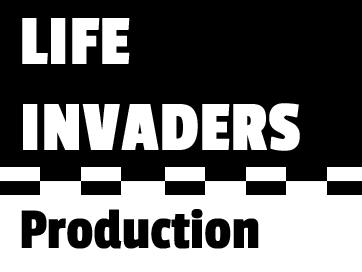
\includegraphics[scale=0.4]{logo_lifeinvaders_copie.png}
    \end{figure}
\end{titlepage}

% ////////////////////////////////////////////////
% ////////////////////////////////////////////////
% ////////////////////////////////////////////////


\tableofcontents
\newpage

\pagestyle{fancy}
\lhead{Panic At Tortuaga}
\fancyhead[C]{Février 2021}
\rhead{LifeInvaders Production}

\section{Introduction}

Panic At Tortuga est un jeu orienté multijoueur. Mais quel genre de est-ce ?
Il s'agit du jeu s'inspirant de mécaniques de jeux divers, 
les principaux étant Assassin's Creed (son mode multi) et d'autres jeux comme "Guess Who?".

Vous et d'autres joueurs êtes lachés sur la petite île de Tortuga, une île où la population vit paisiblement.
Mais parmi eux, déguisés, se cachent des pirates sanguinaires, et c'est à vous de les éliminer.

Le début de production de notre équipe de dévellopement, Lifeinvaders Production,
composé de Paul, Harrys, Julien et Dov; a pu commencer à développer le jeu depuis mi-décembre.
Nous avons pu apprendre de nombreuses choses, se dépaser, sortir de notre zone de confort, mais surtout prendre du plaisir à créer notre jeu !

% ////////////////////////////////////////////////
% ////////////////////////////////////////////////
% ////////////////////////////////////////////////

\section{Conception}

    Le concept de notre jeu se base sur une idée simple : Vous avez une cible et êtes celle d'un autre joueur.
    Vous devez éliminer chaque cible attribué (en l'occurence d'autres joueurs) et tenter de survivre dans ce petit archipel.

    Nous nous sommes répartis les taches rapidement les différentes tâches pour avoir les bases.
    Par exemple, le déplacement du personnage et de la caméra était primordial pour Harrys et Julien qui s'occupaient du multijoueur et nécéssitait d'être livré rapidement.
    Pendant que Renaud-Dov réalisait l'implémentation de ces scripts, Julien et Harrys ont commencé à apprendre comment fonctionnait Photon. Paul s'occupait alors de la map.

    Pour éviter de se perdre dans l'afflux de tâches à réaliser, nous décidé d'utiliser des
    outils de travail en équipe tel que des kanban (avec Github Projects).\\
    
    % Photo du kanban

    \begin{figure}[hbt!]
        \centering
        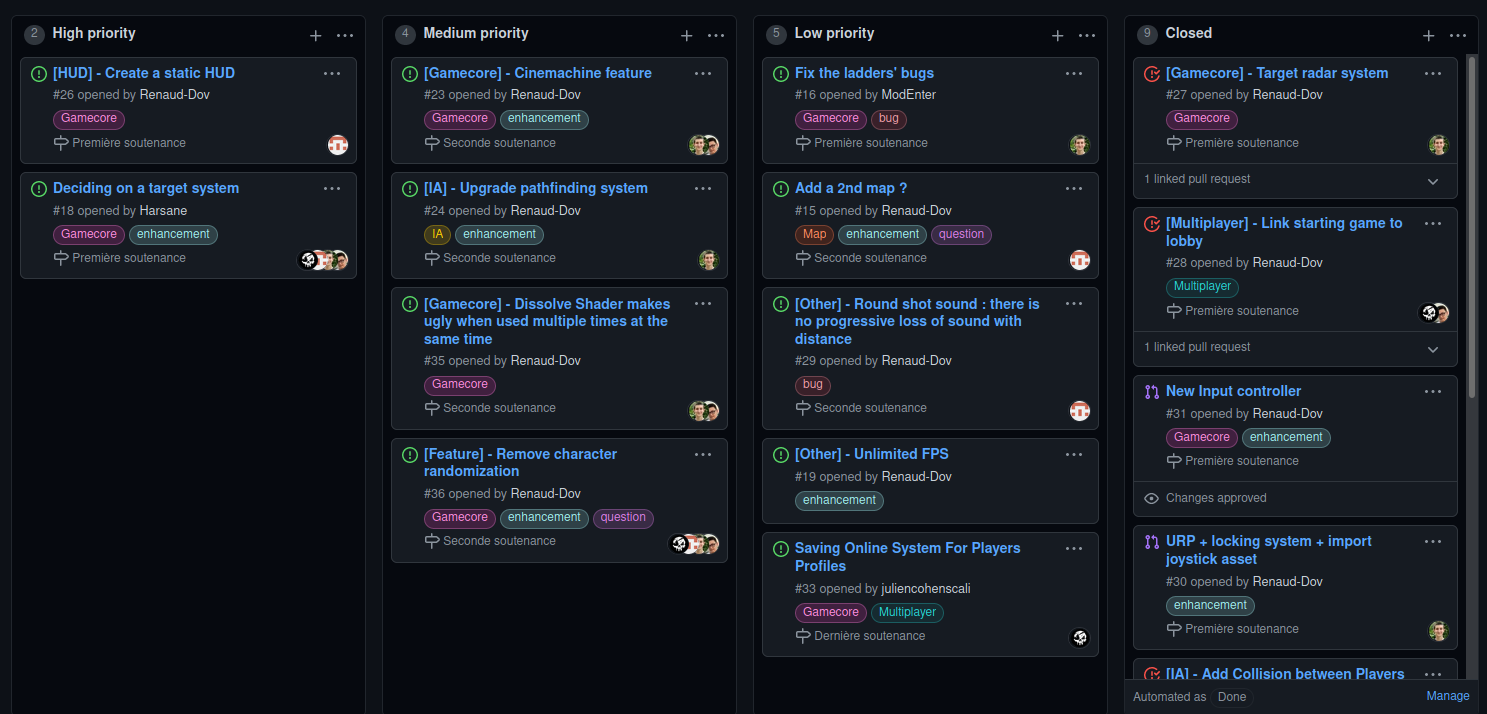
\includegraphics[scale=0.28]{kanban.png}
        \caption{Kanban pour la priorisation des tâches sur Github}
    \end{figure}


    % ////////////////////////////////////////////////
    % ////////////////////////////////////////////////
    % ////////////////////////////////////////////////
    
    \subfile{sections/reseau.tex}
    \newpage
    % ////////////////////////////////////////////////
    % ////////////////////////////////////////////////
    % ////////////////////////////////////////////////

    \subfile{sections/ia.tex}


    % ////////////////////////////////////////////////
    % ////////////////////////////////////////////////
    % ////////////////////////////////////////////////

    \subfile{sections/gameplay.tex}
    \newpage

    % ////////////////////////////////////////////////
    % ////////////////////////////////////////////////
    % ////////////////////////////////////////////////

    \subsection{Interface}
    
    Les interfaces sont une partie importante de tout jeu. Elles permettent de donner au joueur plus de contrôle sur son expérience et de présenter les informations nécessaires de façon claire, facilement accessible et si possible esthétique. Un progrès important a été fait quant à la création d'interfaces.

        \subsubsection{HUD}
        \subfile{sections/hud.tex} % sous-partie dans HUD.tex
        \subsubsection{Menu principal}
        \subfile{sections/menus.tex}
        \newpage


    % ////////////////////////////////////////////////
    % ////////////////////////////////////////////////
    % //////////////////////////////////////////////// 
    \subfile{sections/map.tex}
    % ////////////////////////////////////////////////
    % ////////////////////////////////////////////////
    % //////////////////////////////////////////////// 
    \subfile{sections/progression.tex}
    

% ////////////////////////////////////////////////
% ////////////////////////////////////////////////
% ////////////////////////////////////////////////

\subfile{sections/avance.tex}
\subfile{sections/previsions.tex}
% ////////////////////////////////////////////////
% ////////////////////////////////////////////////
% ////////////////////////////////////////////////
% ////////////////////////////////////////////////
% ////////////////////////////////////////////////
% ////////////////////////////////////////////////
\newpage
\listoffigures
\listoftables
\end{document}
